
%----------------------------------------------------------------------------------------
%	PACKAGES AND OTHER DOCUMENT CONFIGURATIONS
%----------------------------------------------------------------------------------------

\documentclass[final]{beamer}

\usepackage[scale=1.24]{beamerposter} % Use the beamerposter package for laying out the poster

\usepackage{algorithm,algorithmic}
\usepackage{url}

\usetheme{confposter} % Use the confposter theme supplied with this template

\setbeamercolor{block title}{fg=jblue,bg=white} % Colors of the block titles
\setbeamercolor{block body}{fg=black,bg=white} % Colors of the body of blocks
\setbeamercolor{block alerted title}{fg=white,bg=jblue!80} % Colors of the highlighted block titles
\setbeamercolor{block alerted body}{fg=black,bg=jblue!10} % Colors of the body of highlighted blocks
% Many more colors are available for use in beamerthemeconfposter.sty

%-----------------------------------------------------------
% Define the column widths and overall poster size
% To set effective sepwid, onecolwid and twocolwid values, first choose how many columns you want and how much separation you want between columns
% In this template, the separation width chosen is 0.024 of the paper width and a 4-column layout
% onecolwid should therefore be (1-(# of columns+1)*sepwid)/# of columns e.g. (1-(4+1)*0.024)/4 = 0.22
% Set twocolwid to be (2*onecolwid)+sepwid = 0.464
% Set threecolwid to be (3*onecolwid)+2*sepwid = 0.708

\newlength{\sepwid}
\newlength{\halfcolwid}
\newlength{\onecolwid}
\newlength{\twocolwid}
\newlength{\threecolwid}
\setlength{\paperwidth}{48in} % A0 width: 46.8in
\setlength{\paperheight}{36in} % A0 height: 33.1in
\setlength{\sepwid}{0.02\paperwidth} % Separation width (white space) between columns
\setlength{\halfcolwid}{0.13\paperwidth} % Width of one column
\setlength{\onecolwid}{0.3\paperwidth} % Width of one column
\setlength{\twocolwid}{0.464\paperwidth} % Width of two columns
\setlength{\threecolwid}{0.708\paperwidth} % Width of three columns
\setlength{\topmargin}{-0.6in} % Reduce the top margin size
%-----------------------------------------------------------

\usepackage{graphicx}  % Required for including images

\usepackage{booktabs} % Top and bottom rules for tables

%----------------------------------------------------------------------------------------
%	TITLE SECTION 
%----------------------------------------------------------------------------------------

\title{Web page comparison on post-load DOM trees} % Poster title

\author{Jonathan Thomas (Honors Capstone), Ayush Goel and Prof. Harsha Madhyastha} % Author(s)

\institute{University of Michigan} % Institution(s)

%----------------------------------------------------------------------------------------

\begin{document}

\addtobeamertemplate{block end}{}{\vspace*{0.5ex}} % White space under blocks
\addtobeamertemplate{block alerted end}{}{\vspace*{0.5ex}} % White space under highlighted (alert) blocks

\setlength{\belowcaptionskip}{0.5ex} % White space under figures
\setlength\belowdisplayshortskip{0.5ex} % White space under equations

\begin{frame}[t] % The whole poster is enclosed in one beamer frame

\begin{columns}[t] % The whole poster consists of three major columns, the second of which is split into two columns twice - the [t] option aligns each column's content to the top

\begin{column}{\sepwid}\end{column} % Empty spacer column

\begin{column}{\onecolwid} % The first column

%----------------------------------------------------------------------------------------
%	OBJECTIVES
%----------------------------------------------------------------------------------------

\begin{alertblock}{Problem}
Code is always being rewritten and in constant need of further improvement. As such, source code for web pages changes drastically over time, and it is important to know what it really means for a web page to be the same as another or the same as a previous version of itself. In order to proceed, we introduce a core browser concept.

\begin{columns}
\begin{column}{\halfcolwid}
The main entity we are concerned with is the Document Object Model (DOM) tree, which keeps track of the structure of the web page at a high level and is modified as the page loads. 
\end{column}

\begin{column}{\halfcolwid} % Begin a column which is two columns wide (column 2)
\begin{figure}
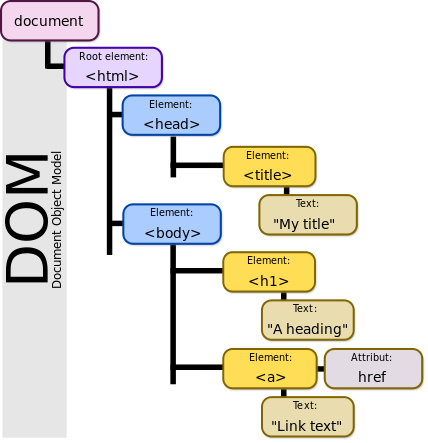
\includegraphics[width=0.6\linewidth]{dom.png}
\caption{An example DOM}
\end{figure}
\end{column}
\end{columns}
There is a need for an approach and implementation of a more useful way to check differences between two web pages than a naive diff of the source code text. We also wish to get a better understanding of how the DOM differs over different sites as well as environments, which will be explained below.
\end{alertblock}

%----------------------------------------------------------------------------------------
%	OBJECTIVE
%----------------------------------------------------------------------------------------

\begin{block}{Objective}
In this project, I wrote a tool to determine how similar two web pages are from the perspective of a user visiting either page. This was achieved by comparing the resulting post-load DOM trees of loading two web pages and quantifying how similar they were. Using this tool, we aim to form a better idea of how real web pages change over time. 

The major steps for this project included:
\begin{itemize}
    \item Navigating to a site and dumping the DOM after loading.
    \item Comparing two loads and reporting the differences.
    \item Automating the process across several websites and graphing results.
\end{itemize}
\end{block}

%----------------------------------------------------------------------------------------
%	METHODS
%----------------------------------------------------------------------------------------
\vspace{-0.5cm}
\begin{block}{Methodology}
To evaluate the appearance of the DOM in addition to the structure, we make a first pass over the source code and serialize the computed CSS styles into the DOM. We also make use of a more discerning algorithm for comparison than a naive tree diff. 

In addition to comparing two loads of the same web page in a standard live setup, we wanted to explore how the DOM changes in a replay environment using the mahimahi tool \cite{netravali_sivaraman_winstein_das_goyal_balakrishnan_2014}. After recording replay data for $\sim 100$ websites randomly chosen from the Alexa top 1000, we performed the comparison within these replay environments. We also constructed modified versions of the replay environments by manually removing sources of non-determinism from any included JavaScript files. 
\end{block}

%----------------------------------------------------------------------------------------

\end{column} % End of the first column

\begin{column}{\sepwid}\end{column} % Empty spacer column

\begin{column}{\onecolwid} % Begin a column which is two columns wide (column 2)

%----------------------------------------------------------------------------------------
%	RESULTS
%----------------------------------------------------------------------------------------

\begin{block}{Results}

First, we justify why a smarter DOM comparison is necessary. The following graph compares the differences detected in a naive algorithm vs. our algorithm in comparing a suite of live web pages.

\begin{figure}
\vspace{0.5cm}
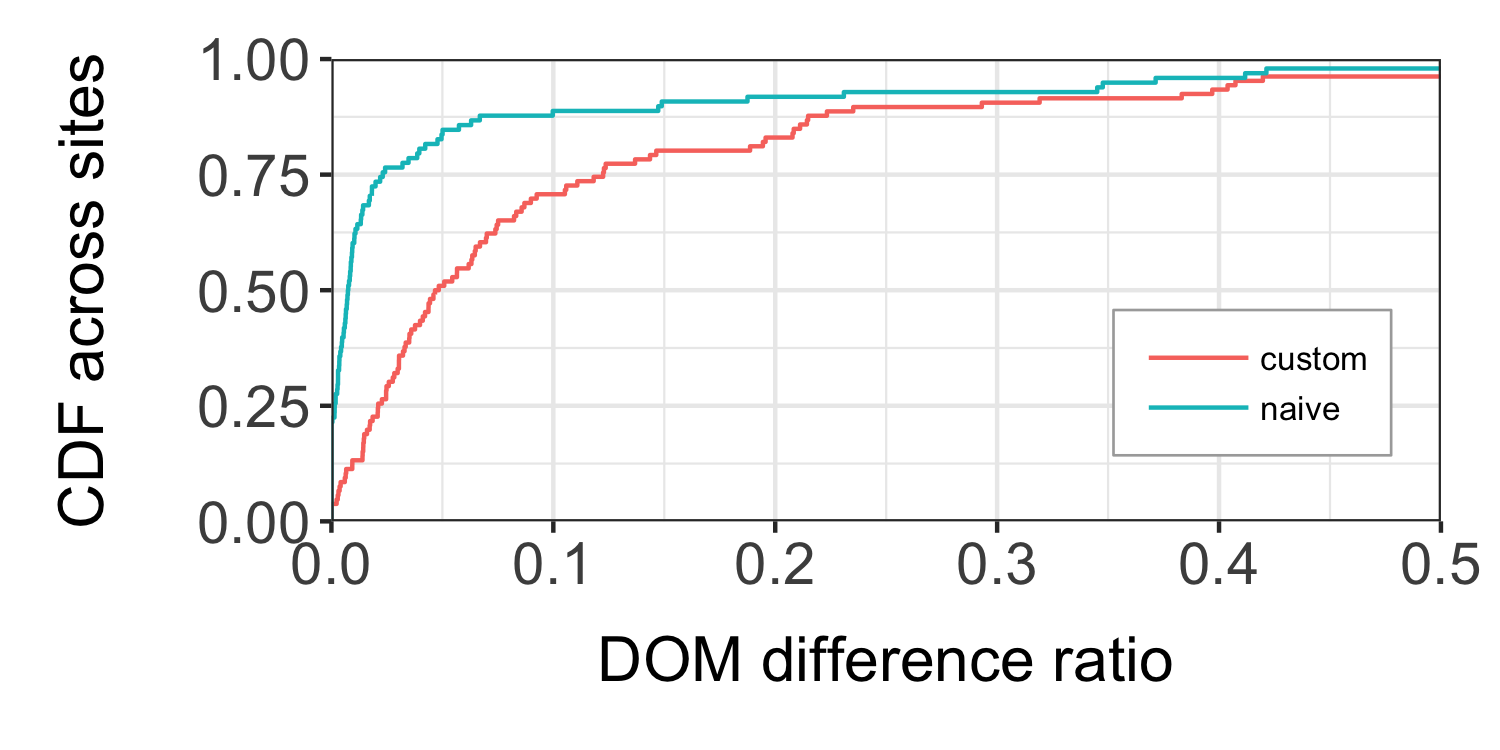
\includegraphics[width=0.8\linewidth]{naive_comparison_plot.png}
\vspace{-1.5cm}
\caption{How our comparison performs compared to a naive approach}
\end{figure}

As seen, our approach identifies many additional differences that the naive approach suppresses to determine if a web page has changed. 

Having established the viability of this approach, we now compare the differences between the three classes of comparisons: comparison with live loads, loads within a replay environment, and finally loads within a modified replay environment.

\begin{figure}
\vspace{0.5cm}
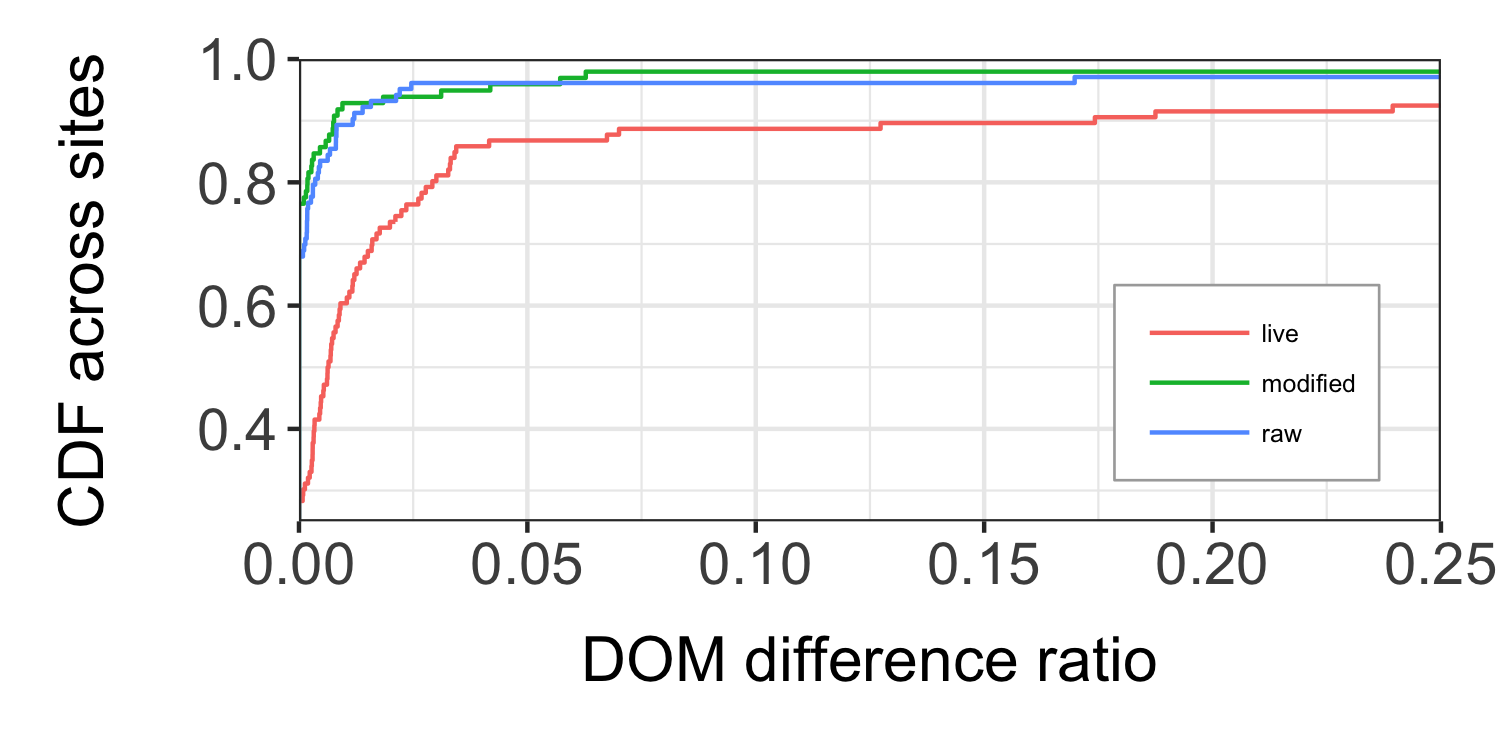
\includegraphics[width=0.8\linewidth]{dom_plot.png}
\vspace{-1.5cm}
\caption{DOM comparison across environments}
\end{figure}

We can see that the DOM differs significantly more in the live loads than those done in a replay environment.

Finally, we show how the logged network requests change across the different environments for reference.

\begin{figure}
\vspace{0.5cm}
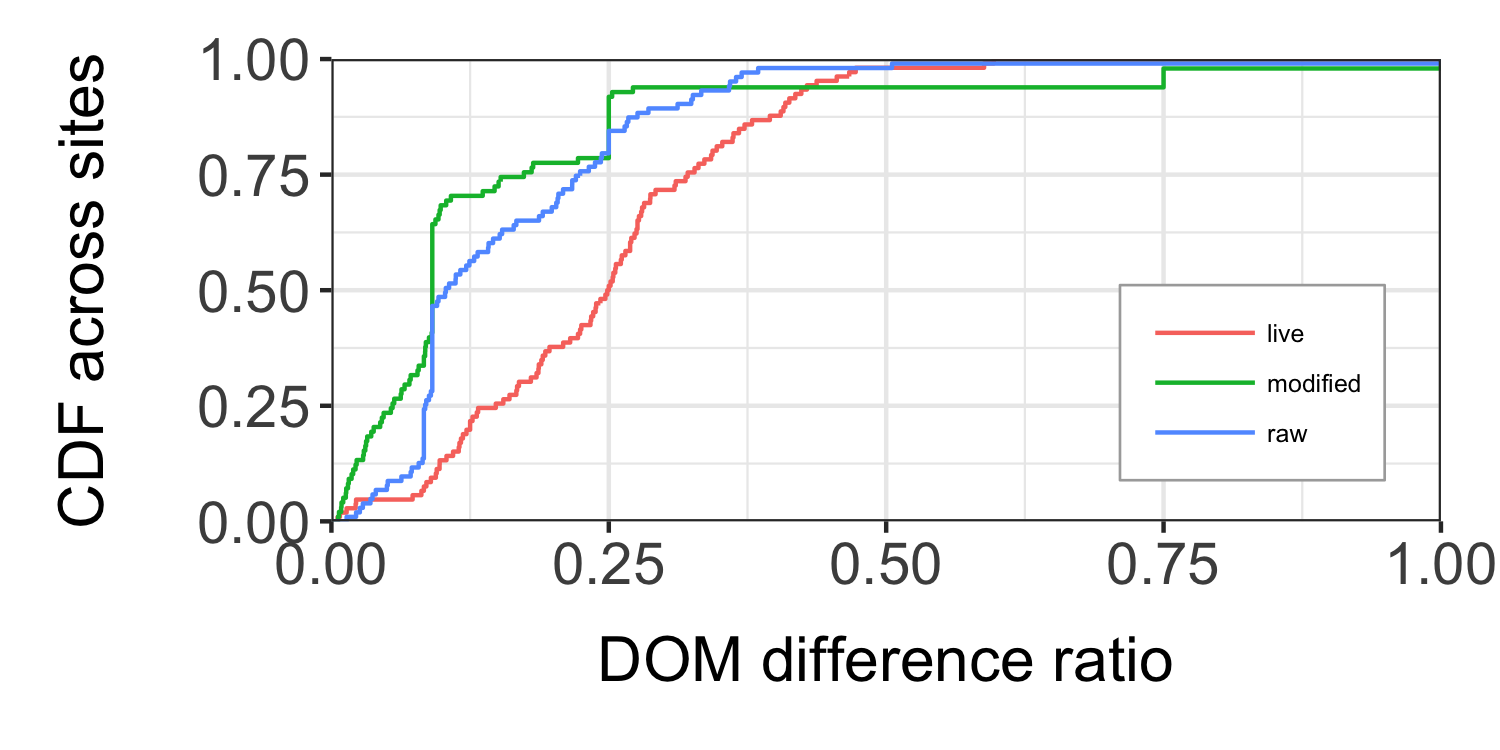
\includegraphics[width=0.8\linewidth]{network_plot.png}
\vspace{-1.5cm}
\caption{Network request comparison across environments}
\end{figure}

\end{block}

%----------------------------------------------------------------------------------------

\end{column} % End of the second column

\begin{column}{\sepwid}\end{column} % Empty spacer column

\begin{column}{\onecolwid} % The third column

%----------------------------------------------------------------------------------------
%	DISCUSSION
%----------------------------------------------------------------------------------------

\begin{block}{Discussion}

The results show that almost all live web pages sampled change across back-to-back loads with this comparison. Existing work suggested a general trend of only roughly 22\% of websites having the same DOM structure on back to back loads \cite{ruamviboonsuk_netravali_uluyol_madhyastha_2017}, but this figure did not account for changes in style or attributes of the DOM elements.

Additionally, while the replay environment helps decrease the detected changes in both the DOM  and the network requests sent, there are still sources of non-determinism that cause changes. In the modified replay environments supplied, we see less change, but there are still sources of differences present that are currently being investigated. 

\end{block}

%----------------------------------------------------------------------------------------
%	CONCLUSION
%----------------------------------------------------------------------------------------

\begin{block}{Next Steps}

Some areas for future exploration include optimization of the existing tool, a better characterization of the types of differences that appear, and extension of the modified replay environment to account for more sources of non-determinism.  

This tool can also be applied in web page optimization research, where it could be used to evaluate the correctness of existing work. Rewriting source code is common in this field to gain improvements in speed and memory usage. This project would provide useful information to determine how users' modifications have affected the content of the rewritten web pages.
\end{block}

%----------------------------------------------------------------------------------------
%	REFERENCES
%----------------------------------------------------------------------------------------

\begin{block}{References}
\vspace{-0.5cm}
\nocite{*} % Insert publications even if they are not cited in the poster
\footnotesize{\bibliographystyle{unsrt}
\bibliography{capstone}}

\end{block}

%----------------------------------------------------------------------------------------
%	ACKNOWLEDGEMENTS
%----------------------------------------------------------------------------------------

%\setbeamercolor{block title}{fg=red,bg=white} % Change the block title color

%----------------------------------------------------------------------------------------
%	CONTACT INFORMATION
%----------------------------------------------------------------------------------------

\begin{alertblock}{Acknowledgements}

\small{\rmfamily{I would like to thank Prof. Harsha Madhyastha, Ayush Goel, and the Engineering Honors Program for mentorship and guidance throughout this project.
}} \\

\begin{itemize}
\item Email: \href{mailto:jonthoma@umich.edu}{jonthoma@umich.edu}
\end{itemize}
\end{alertblock}

\vspace{-2.5cm}
\begin{center}
\begin{figure}

\includegraphics[width=0.45\linewidth]{CoE-Honors-vert.png}
\end{figure}
\end{center}

%\begin{columns}
%\begin{column}{\halfcolwid}
%\begin{figure}
%\includegraphics[width=\linewidth]{logo.png}
%\caption{Replace with EECS logo}
%\end{figure}
%\end{column}

%\begin{column}{\halfcolwid} % Begin a column which is two columns wide (column 2)
%\begin{figure}
%
\includegraphics[width=\linewidth]{CoE-Honors-vert.png}
%\end{figure}
%\end{column}
%\end{columns}

%----------------------------------------------------------------------------------------

\end{column} % End of the third column

\end{columns} % End of all the columns in the poster

\end{frame} % End of the enclosing frame

\end{document}
